% Adapted from the CMMR 2025 paper with minimal changes for thesis Chapter 3.
% Main changes: shortened generic introduction/related-work material,
% preserved core method/experiments/results, and added a thesis-oriented discussion.
\newcommand{\eqshift}{\qquad\qquad\qquad\qquad}

\chapter{Symbolic MIDI Velocity Completion as Image Colorization}
\label{ch:velcomp}

\noindent\textbf{Source and adaptation note.}
This chapter is adapted from the CMMR 2025 paper \cite{he2025filling}.
Relative to the published version, the thesis chapter shortens the general introduction and literature survey already covered in Chapter~\ref{ch:introduction} and Chapter~\ref{ch:background}, while keeping the technical method, experimental protocol, and main findings largely unchanged.

\section{Chapter Overview and Position in the Thesis}
\label{sec:velcomp:overview}

This chapter is the first paper-based method chapter of the thesis. It addresses Scenario~S1, the most controlled setting in the thesis map. Here the symbolic notes and their timing are already known, but the note-level velocity is missing, flattened, or musically uninformative. The chapter therefore asks a focused question: can useful note-level dynamics be recovered from symbolic structure alone, without changing the original composition?

This setting matters because it isolates the dynamics problem from the broader transcription problem. It is common in digital audio workstation workflows, step-entered MIDI, quantized MIDI, and corpus curation settings where note content already exists but expression does not. It also provides the cleanest test of the thesis claim that dynamics can be treated as a separate and editable target rather than as a side effect of full expressive performance generation.

In thesis terms, this chapter makes three contributions. First, it shows that symbolic velocity completion can be formulated naturally as an image-colorization problem on sparse piano-roll representations. Second, it develops a U-Net-based model with window attention and a sparsity-aware loss tailored to this representation. Third, it provides both objective and perceptual evidence that recovering only MIDI velocity can improve musical expressiveness in a controlled setting.

\section{Task-Specific Related Work}
\label{sec:velcomp:related}

MIDI velocity completion sits at the intersection of expressive rendering and symbolic refinement. Broad expressive-rendering systems often predict timing, articulation, and dynamics jointly \cite{jeong2019virtuosonet,borovik2023scoreperformer}. These systems are important, but they are not ideal when the practical goal is to preserve a user's note content and timing while improving only intensity. A velocity-only formulation is narrower, but it is also more controllable.

Recent symbolic velocity-prediction methods have typically treated the task as sequential prediction. Representative examples include convolutional autoencoders and sequence-to-sequence models with attention \cite{kuo2021velocity,kim2023piano}. These models establish that note-level velocity can be learned from symbolic context. However, piano-roll data is sparse and polyphonic. The relevant structure is not only sequential. It is also spatial. Simultaneous notes create meaningful vertical patterns, and short local pitch--time neighborhoods often carry clear expressive cues.

This motivates the image-based view adopted in the present chapter. By treating symbolic MIDI as a sparse image and velocity as a colorization target, the model can exploit local polyphonic structure more directly. U-Net and attention mechanisms are already successful in related music and audio tasks, but the present setting is distinct because it is purely symbolic and does not rely on acoustic input \cite{he2025filling,kim2024method}. This makes the chapter a natural starting point for the broader thesis.

\section{Problem Setting}
\label{sec:velcomp:problem}

MIDI (Musical Instrument Digital Interface) is the dominant symbolic format in modern music production.
A MIDI file that resembles sheet music can still sound mechanical when its note velocities are undefined or flattened to a default constant.
In contrast, MIDI captured from human performance preserves the performer's control of intensity and therefore carries a substantial portion of the perceived musical expression.
As discussed in the thesis introduction, dynamics is the expressive dimension targeted first in this thesis because it is both perceptually salient and directly editable.
This chapter studies the most constrained setting in that map: recovering note-level MIDI velocity when the symbolic notes and their timing are already known.

\begin{figure}[t]
\begin{center}
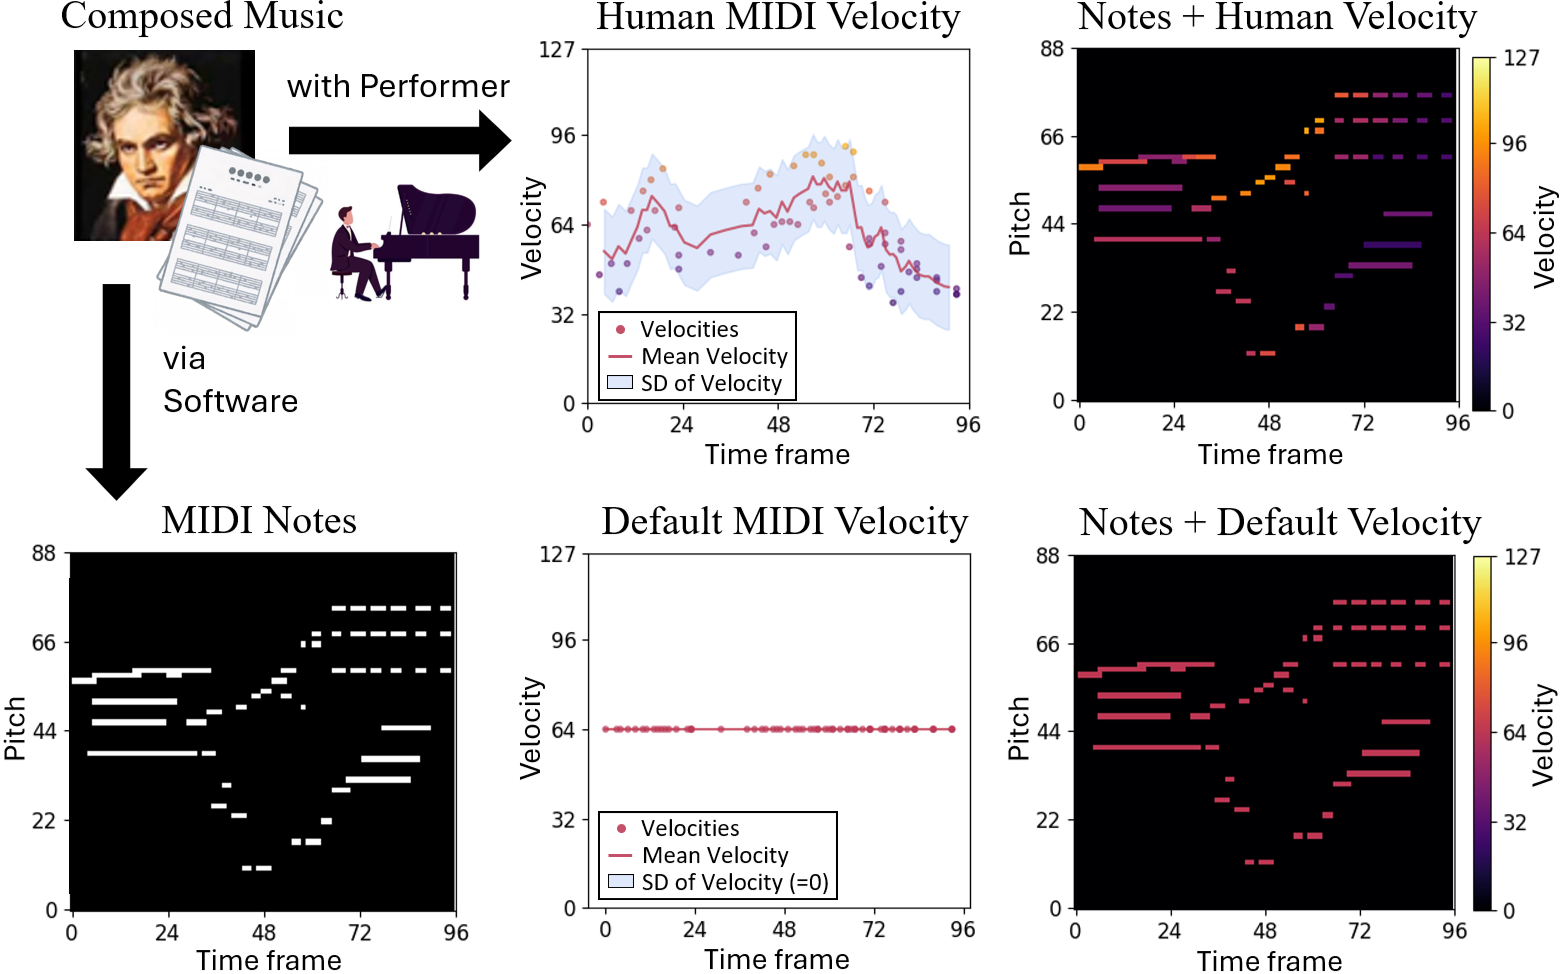
\includegraphics[width=0.86\textwidth]{Chapter_3/figures/p1.png}
\caption{Comparison between MIDI notes with human-performed velocity and music-software default velocity (64 when unspecified). The standard deviation of velocity (\(SD_{\text{velo}}\)) represents the dispersion of velocities around their mean across pitches.}
\label{fig:velcomp_intro}
\end{center}
\end{figure}

This setting is practically important for two reasons.
First, a large amount of MIDI used in digital audio workstation workflows is created by step input, quantization, or low-cost controllers, leaving velocity flat.
Second, many expressive rendering systems modify several performance dimensions jointly, including timing and sometimes note content, which is undesirable when the goal is to preserve the user's composition.
By isolating velocity, the task becomes a precise and controllable refinement problem: the notes, onsets, and offsets remain fixed, and only note intensity is completed.

Chapter~\ref{ch:background} reviewed prior symbolic velocity-prediction methods, most of which formulate the problem sequentially.
The key design choice in this chapter is instead to exploit the spatial structure of polyphonic symbolic music by treating MIDI as an image-colorization problem.
MIDI without velocity is represented as a binary pianoroll, while the target is a velocity-valued pianoroll.
This formulation is especially natural for instruments such as piano, where multiple simultaneous notes create rich vertical patterns.
Current dataset availability restricts the experiments here to piano data, but the formulation itself is not tied to piano alone.

\section{Representation as Image-like MIDI Matrices}
\label{sec:velcomp:representation}

\subsection{Matrix Representation}
\label{sec:velcomp:matrix}

To process MIDI as images, we convert each performance into three matrices of size \(T \times P\), where \(T\) is the number of time frames and \(P=88\) is the number of piano pitches.
The three matrices are a binary onset roll \(O\), marking note starts; a binary frame roll \(F\), indicating note activation over time; and a velocity roll \(V\), acting as the target color intensity.
In the implemented system, \(F\) is the network input, \(V\) is the prediction target, and \(O\) is used for onset masking in the loss.
For the velocity roll, integer values in \([0,127]\) are normalized to \([0,1)\) to match the model output activation range.
During post-processing, the model output is denormalized by scaling and rounding back to integer MIDI velocity.
As illustrated in Figure~\ref{fig:velcomp_model}, these matrices are highly sparse.

\subsection{MIDI Segmentation}
\label{sec:velcomp:segmentation}

The segment duration is a key design variable in this formulation.
Because a MIDI performance often exceeds three minutes, we split each piece into shorter segments to keep the computation tractable.
The number of time frames \(T\) determines the temporal granularity of the matrix representation, so the timestep resolution is
\begin{equation}
\text{Resolution} = \frac{\text{Segment Duration}}{T}.
\label{eq:velcomp_resolution}
\end{equation}
Unlike tasks that require fine temporal resolution to detect unknown note events, the present task already assumes that note timing is given.
This makes a more computationally efficient timestep resolution feasible.
With a fixed input size of \(T=96\), we explored segment durations of 5 s, 10 s, 15 s, and 20 s in hyperparameter search and found that 10 s yielded the best results.
A plausible explanation is that a 10-second window often captures a musically coherent phrase, for example roughly four measures at 120 BPM, providing enough context without overextending the receptive field.

\begin{figure}[t]
\begin{center}
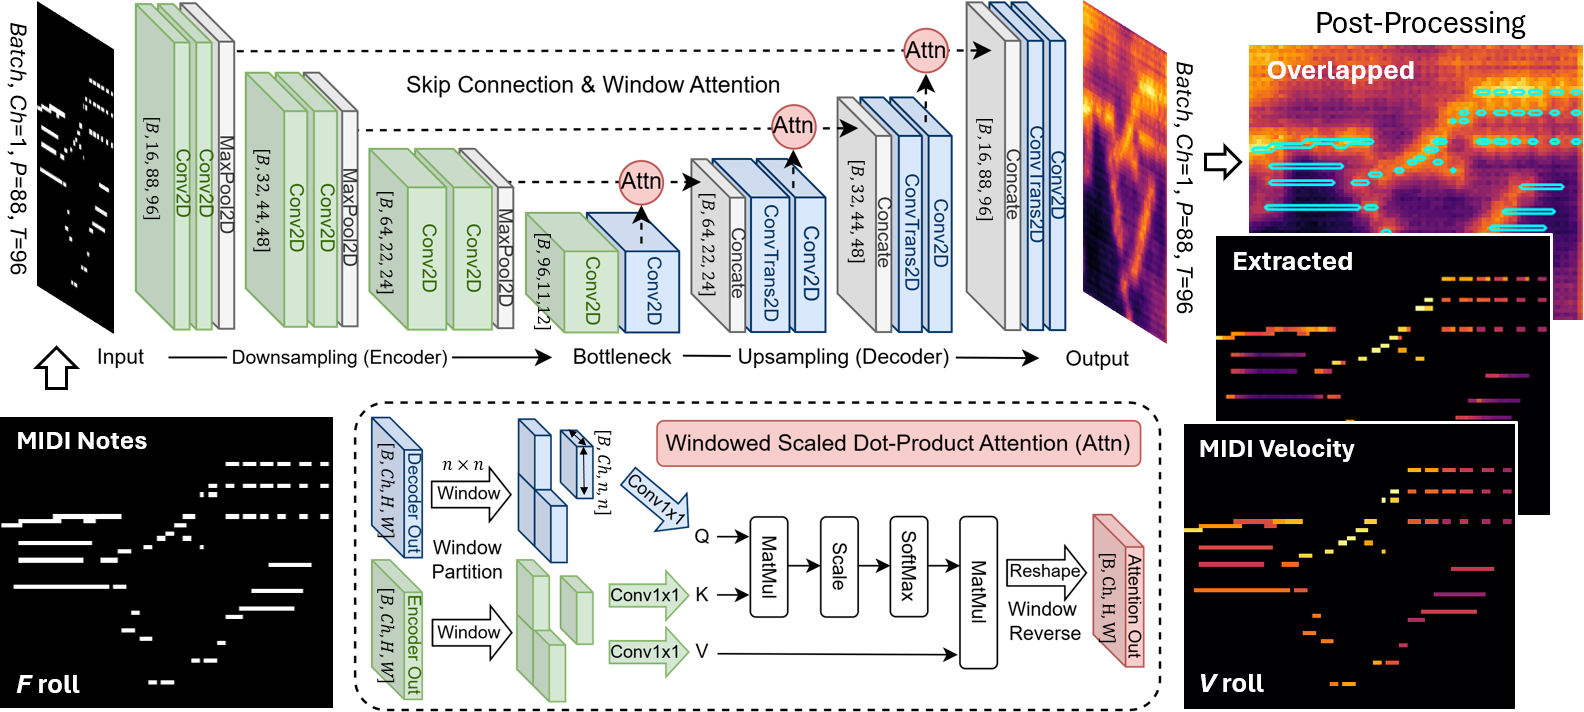
\includegraphics[width=\textwidth]{Chapter_3/figures/p2.png}
\caption{Proposed U-Net architecture. The model input (\(F\) roll) comprises 88 pitch bins and 96 time frames. Attn block denotes windowed scaled dot-product attention. The final velocity roll (\(V\) roll) is generated during post-processing by extracting velocity at note positions and assigning each note the velocity at its onset.}
\label{fig:velcomp_model}
\end{center}
\vspace{-12pt}
\end{figure}

\section{Model Architecture and Loss}
\label{sec:velcomp:model}

\subsection{U-Net with Window Attention}
\label{sec:velcomp:architecture}

The proposed architecture is shown in Figure~\ref{fig:velcomp_model}.
The U-Net extracts higher-level features through downsampling, while skip connections preserve local details together with broader structural patterns.
All convolution blocks use \(3 \times 3\) kernels, stride 1, and padding 1, followed by sigmoid activation and batch normalization.
Downsampling is implemented with a standard \(2 \times 2\) MaxPool2D layer.
For upsampling, we use transpose convolutions with \(4 \times 4\) kernels and stride 2, following the image-colorization variant in \cite{wang2022cunet}.

To address MIDI sparsity, we insert windowed scaled dot-product attention (window attention) \cite{shen2023linear} into the U-Net.
Traditional self-attention \cite{vas2017attn} operates on the full feature map \(X \in \mathbb{R}^{H \times W}\), where \(H\) and \(W\) denote height and width.
Window attention instead partitions \(X\) into non-overlapping \(n \times n\) windows and computes attention within each window.
This reduces computational complexity while still improving feature aggregation \cite{chen2022hts}.

The window size \((n)\) balances local detail against broader dependency modeling.
We explored \(n \in \{1, 2, 4, 8\}\) and found that \(2 \times 2\) window attention performed best in hyperparameter search.
This suggests that attention is useful in this sparse setting, but overly large windows can compress information too aggressively and reduce effectiveness.

\subsection{Sparsity-aware Loss Function}
\label{sec:velcomp:loss}

The proposed loss combines binary cross-entropy (BCE) with cosine similarity (CosSim), following \cite{kim2023piano}, with \(\alpha = 0.2\):
\begin{equation}
\mathcal{L}_{\mathrm{Combine}} = (1-\alpha)\,\mathcal{L}_{\mathrm{BCE}} + \alpha\,\left(1-\mathrm{CosSim}\right).
\label{eq:velcomp_loss_combine}
\end{equation}
Here BCE optimizes element-wise prediction error, while CosSim is computed pitch-wise and then averaged to capture the trend of velocity variation over time:
\begin{gather}
\mathrm{CosSim} = \frac{1}{P}\sum_{p=1}^{P}
\frac{\sum_{t=1}^{T} y_{t,p}\,\hat{y}_{t,p}}
{\sqrt{\sum_{t=1}^{T} y_{t,p}^{2}}\;\sqrt{\sum_{t=1}^{T} \hat{y}_{t,p}^{2}}},
\label{eq:velcomp_cossim}\\
\mathcal{L}_{\mathrm{BCE}} = \frac{1}{TP}\sum_{t=1}^{T}\sum_{p=1}^{P}
l_{\mathrm{bce}}\!\left(y_{t,p}, \hat{y}_{t,p}\right).
\label{eq:velcomp_bce}
\end{gather}
In these expressions, \(y_{t,p}\) and \(\hat{y}_{t,p}\) denote the target and predicted velocity, respectively, and \(t\) and \(p\) index time and pitch.

To better match the structure of the task, we introduce two modifications.
First, a masking operation \(<m>\) based on the onset roll \(O\) ignores silent time steps and counts each note once at its onset.
Second, a weighting operation \(<w>\) emphasizes the velocity-range boundaries, which are harder to predict accurately \cite{jeong2020note,kim2024method,kim2023score}.
Motivated by the approximately Gaussian velocity distribution in Figure~\ref{fig:velcomp_data_dist}, we use a V-shaped weighting centered on 64 (normalized to 0.5), with empirical factor 3:
\begin{equation}
\mathcal{L}_{\mathrm{BCE}}^{<m,w>} = \frac{1}{TP}\sum_{t=1}^{T}\sum_{p=1}^{P}
O_{t,p}\,\bigl(1 + 3\lvert V_{t,p} - 0.5 \rvert\bigr)\,l_{\mathrm{bce}}\!\left(y_{t,p}, \hat{y}_{t,p}\right).
\label{eq:velcomp_bce_weighted}
\end{equation}
The final objective replaces \(\mathcal{L}_{\mathrm{BCE}}\) in Eq.~\eqref{eq:velcomp_loss_combine} with \(\mathcal{L}_{\mathrm{BCE}}^{<m,w>}\).
This loss focuses learning on note onsets while also penalizing the underestimation of more extreme dynamic values.

\section{Experimental Setup}
\label{sec:velcomp:experiment}

\subsection{Datasets}
\label{sec:velcomp:datasets}

For training, we use the MAESTRO v3.0.0 dataset \cite{hawthorne2019maestro}, recorded by skilled pianists on Yamaha Disklavier pianos during the International Piano-e-Competition.
The default train/validation/test split is used.
With 1,276 performances totaling more than 200 hours, MAESTRO provides a strong foundation for modeling MIDI velocity.

For evaluation, we use the Saarland Music Data (SMD) dataset \cite{smd}, which contains 50 further performances recorded on a Yamaha Disklavier.
We selected SMD for cross-dataset evaluation instead of the Piano-e-Competition dataset used in \cite{kuo2021velocity,kim2023piano}, because the latter has substantial performance overlap with MAESTRO.
The suitability of SMD is supported by the similar distributional statistics in Figure~\ref{fig:velcomp_data_dist}.
In addition, SMD is used for the subjective listening test, with eight selected performances listed in Table~\ref{tab:velcomp_composers}.
Because SMD overlaps with MAESTRO in composer style but not in exact performances, it allows us to test both familiar and less familiar musical styles.

\begin{figure}[t]
\centering
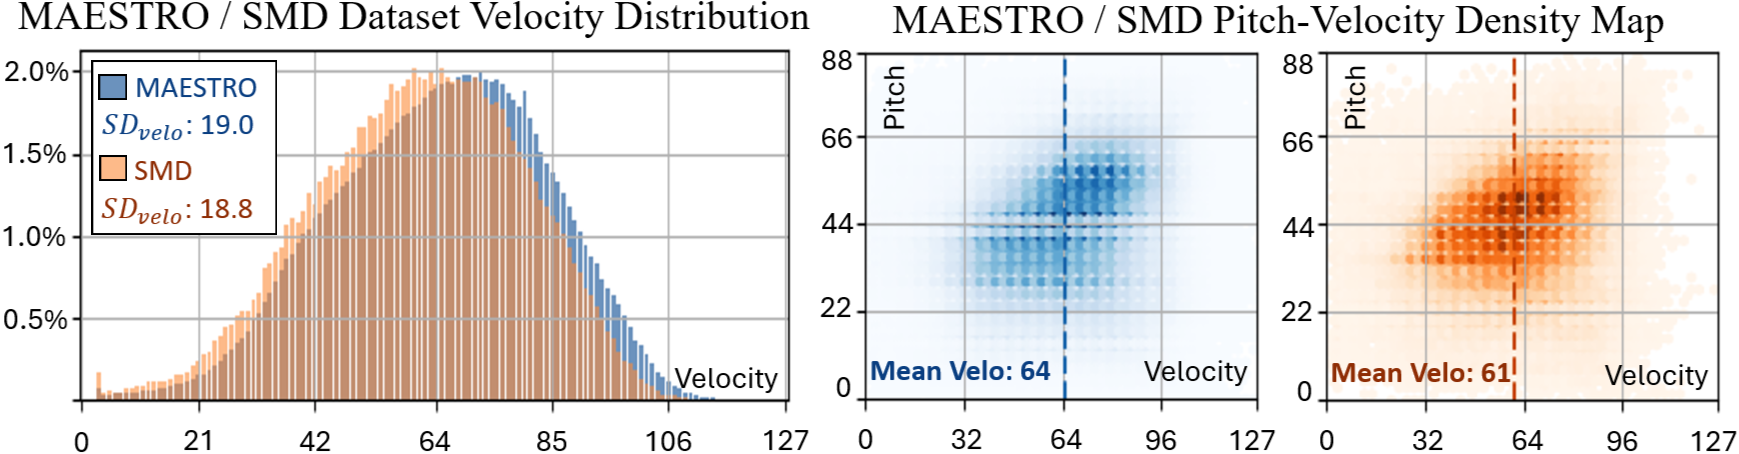
\includegraphics[width=0.96\textwidth]{Chapter_3/figures/p3.png}
\caption{MIDI data distributions of the MAESTRO (blue) and SMD (orange) datasets, with density maps highlighting the similarity in their MIDI feature correlations.}
\label{fig:velcomp_data_dist}
\end{figure}


\begin{table}[t]
\centering
% \scriptsize                        % 控制字体, 把字体切到 LaTeX 预定义的小字号
\setlength{\tabcolsep}{7pt}          % 控制表格列与列之间的左右留白
\fontsize{11pt}{14pt}\selectfont     % 直接设置字体大小和行高
\renewcommand{\arraystretch}{1.2}    % 控制表格行高倍率
\caption{Selected SMD performances for the subjective listening test, together with SMD composer statistics and their overlap with the MAESTRO training set.}
\label{tab:velcomp_composers}
\begin{tabular}{|l|l|l|l|l|}
\hline
& \multicolumn{2}{c|}{\textbf{MAESTRO train set}} & \multicolumn{2}{c|}{\textbf{SMD dataset}} \\
\hline
\textbf{Composer} & \textbf{Total Perf.} & \textbf{Total Dur.} & \textbf{Total Perf.} & \textbf{Selected Perf.} \\
\hline
F. Chopin & 145 & 19.9 h & 13 & Op010-04 \\
J. S. Bach & 114 & 11.2 h & 8 & BWV849-02 \\
L. van Beethoven & 110 & 20.5 h & 7 & Op027No1-01 \\
F. Liszt & 93 & 16.0 h & 3 & - \\
R. Schumann & 33 & 12.4 h & 3 & - \\
\hline
S. Rachmaninoff & 29 & 4.2 h & 3 & Op036-02 \\
J. Haydn & 29 & 3.7 h & 4 & Hob017No4 \\
W. A. Mozart & 27 & 3.9 h & 2 & KV265 \\
A. Scriabin & 22 & 4.1 h & 1 & - \\
J. Brahms & 20 & 6.1 h & 3 & - \\
\hline
B. Bartok & 0 & 0 h & 3 & SZ080-03 \\
M. Ravel & 0 & 0 h & 2 & JeuxDEau \\
\hline
\end{tabular}
\end{table}

\subsection{Training Setup}
\label{sec:velcomp:training}

The trained models include the proposed U-Net and a re-implemented ConvAE baseline \cite{kuo2021velocity}.
Following \cite{zhang2023symbolic}, continuous segments from the same piece are arranged into the same batch in order to preserve local musical continuity during training.
Both models are trained for 300 epochs on the MAESTRO training set with learning rate \(10^{-5}\), batch size 3, and the same loss function.
Training takes approximately 12 hours on an NVIDIA V100 32~GiB GPU using the Ranger21 optimizer.
The top three checkpoints of each model, selected by validation performance on MAESTRO, are then tested on the MAESTRO test split and on SMD for cross-dataset evaluation.

\subsection{Evaluation Metrics}
\label{sec:velcomp:metrics}

\textbf{Objective} All objective metrics are computed on denormalized MIDI velocity in the original range of 0 to 127 after note-level post-processing.
Let \(\mathcal{I}\) denote the set of reference note onsets, and let \(V_i\) and \(\hat{V}_i\) denote the reference and predicted velocity of note \(i\), respectively.
We report mean absolute error (MAE), mean squared error (MSE), standard deviation of absolute error (\(SD_{\mathrm{ae}}\)), Recall\textsubscript{10\%}, and the standard deviation of predicted velocity (\(SD_{\mathrm{velo}}\)):
\begin{flalign}
&\eqshift \mathrm{MAE}
= \frac{1}{|\mathcal{I}|}\sum_{i\in\mathcal{I}} \left|V_i-\hat{V}_i\right|, &&
\label{eq:velcomp_mae}\\
&\eqshift \mathrm{MSE}
= \frac{1}{|\mathcal{I}|}\sum_{i\in\mathcal{I}} \left(V_i-\hat{V}_i\right)^2, &&
\label{eq:velcomp_mse}\\
&\eqshift \mathrm{SD}_{\mathrm{ae}}
= \sqrt{\frac{1}{|\mathcal{I}|}\sum_{i\in\mathcal{I}}
\left(\left|V_i-\hat{V}_i\right|-\mathrm{MAE}\right)^2}, &&
\label{eq:velcomp_sdae}\\
&\eqshift \mathrm{Recall}_{10\%}
= \frac{1}{|\mathcal{I}|}\sum_{i\in\mathcal{I}}
\mathbf{1}\!\left(\left|V_i-\hat{V}_i\right| \le 0.1 \times 127\right), &&
\label{eq:velcomp_recall}\\
&\eqshift \mathrm{SD}_{\mathrm{velo}}
= \sqrt{\frac{1}{|\mathcal{I}|}\sum_{i\in\mathcal{I}}
\left(\hat{V}_i-\bar{\hat{V}}\right)^2}, \quad
\bar{\hat{V}}=\frac{1}{|\mathcal{I}|}\sum_{i\in\mathcal{I}}\hat{V}_i. &&
\label{eq:velcomp_sdvelo}
\end{flalign}
Here \(\mathbf{1}(\cdot)\) is the indicator function.
Recall\textsubscript{10\%} uses an absolute tolerance of 10\% of the full MIDI velocity range.
MAE, MSE, and \(SD_{\mathrm{ae}}\) quantify direct prediction error, whereas \(SD_{\mathrm{velo}}\) summarizes how much dynamic variation the system preserves.
The latter is especially relevant here because a model can obtain moderate average error while still collapsing toward an unnaturally narrow dynamic range.

\textbf{Subjective} To complement the objective metrics, we also conduct a reference-based perceptual evaluation and summarize the listener responses as mean opinion scores (MOS) \cite{series2014mursha}.
The protocol is MUSHRA-inspired rather than a strict implementation of the ITU procedure.
Listeners hear the audio rendered from human-performed velocity as the reference and then rate each system output according to its perceived similarity to that reference.
Ratings are collected with a continuous 0--5 slider whose five labeled intervals correspond to ``bad'', ``poor'', ``fair'', ``good'', and ``excellent'' similarity.
The reported MOS is the average of these scores across listeners and stimuli, and 95\% confidence intervals are reported to show rating consistency.

\section{Quantitative Results}
\label{sec:velcomp:results}

Tables~\ref{tab:velcomp_results_smd} and \ref{tab:velcomp_results_maestro} report the model performance when all trainable systems are trained only on the MAESTRO training set.
The Flat model assigns a fixed velocity of 64, corresponding to the default behavior of common music software.
The Seq2Seq baseline uses pretrained weights from \cite{kim2023piano}, while ConvAE \cite{kuo2021velocity} is re-implemented and trained within the same framework.
Across both test conditions, the proposed U-Net outperforms the comparison systems on all reported objective metrics.

\begin{table}[h]
\centering
% \scriptsize                        % 控制字体, 把字体切到 LaTeX 预定义的小字号
\setlength{\tabcolsep}{5pt}          % 控制表格列与列之间的左右留白
\fontsize{11pt}{13pt}\selectfont     % 直接设置字体大小和行高
\renewcommand{\arraystretch}{1.2}    % 控制表格行高倍率
\caption{Quantitative results on the MAESTRO test set, where \(\uparrow\) and \(\downarrow\) indicate whether higher or lower values are better.}
\label{tab:velcomp_results_maestro}
\begin{tabular}{l|ccccc}
\toprule
\multicolumn{1}{c|}{\multirow{2}{*}{\textbf{Model}}}
& \multicolumn{5}{c}{\textbf{MAESTRO test set}} \\
\cmidrule(l){2-6}
& \textbf{MAE} \(\downarrow\)
& \textbf{MSE} \(\downarrow\)
& \textbf{SD\textsubscript{ae}} \(\downarrow\)
& \textbf{Recall\textsubscript{10\%}} \(\uparrow\)
& \textbf{SD\textsubscript{velo}} \(\uparrow\) \\
\midrule
Flat (all velocities set to 64) & 14.8 & 333.8 & 10.2 & 48.5\% & 0 \\
Seq2Seq \cite{kim2023piano} & 13.5 & 286.1 & 9.9 & 53.8\% & 6.2 \\
ConvAE \cite{kuo2021velocity} (re-implemented) & 12.3 & 250.7 & 9.7 & 59.4\% & 9.7 \\
\textbf{U-Net (proposed)} & \textbf{11.5} & \textbf{226.2} & \textbf{9.4} & \textbf{63.8\%} & \textbf{10.7} \\
\bottomrule
\end{tabular}
\end{table}

\begin{table}[h]
\centering
% \scriptsize                        % 控制字体, 把字体切到 LaTeX 预定义的小字号
\setlength{\tabcolsep}{5pt}          % 控制表格列与列之间的左右留白
\fontsize{11pt}{13pt}\selectfont     % 直接设置字体大小和行高
\renewcommand{\arraystretch}{1.2}    % 控制表格行高倍率
\caption{Quantitative results on the SMD dataset, where \(\uparrow\) and \(\downarrow\) indicate whether higher or lower values are better.}
\label{tab:velcomp_results_smd}
\begin{tabular}{l|ccccc}
\toprule
\multicolumn{1}{c|}{\multirow{2}{*}{\textbf{Model}}}
& \multicolumn{5}{c}{\textbf{SMD dataset}} \\
\cmidrule(l){2-6}
& \textbf{MAE} \(\downarrow\)
& \textbf{MSE} \(\downarrow\)
& \textbf{SD\textsubscript{ae}} \(\downarrow\)
& \textbf{Recall\textsubscript{10\%}} \(\uparrow\)
& \textbf{SD\textsubscript{velo}} \(\uparrow\) \\
\midrule
Flat (all velocities set to 64) & 15.3 & 367.5 & 10.4 & 49.2\% & 0 \\
Seq2Seq \cite{kim2023piano} & 15.1 & 356.9 & 10.9 & 48.8\% & 8.5 \\
ConvAE \cite{kuo2021velocity} (re-implemented) & 12.5 & 258.1 & 9.6 & 58.5\% & 9.8 \\
\textbf{U-Net (proposed)} & \textbf{11.2} & \textbf{217.5} & \textbf{9.2} & \textbf{65.1\%} & \textbf{11.1} \\
\bottomrule
\end{tabular}
\end{table}


\begin{figure}[h]
\begin{center}
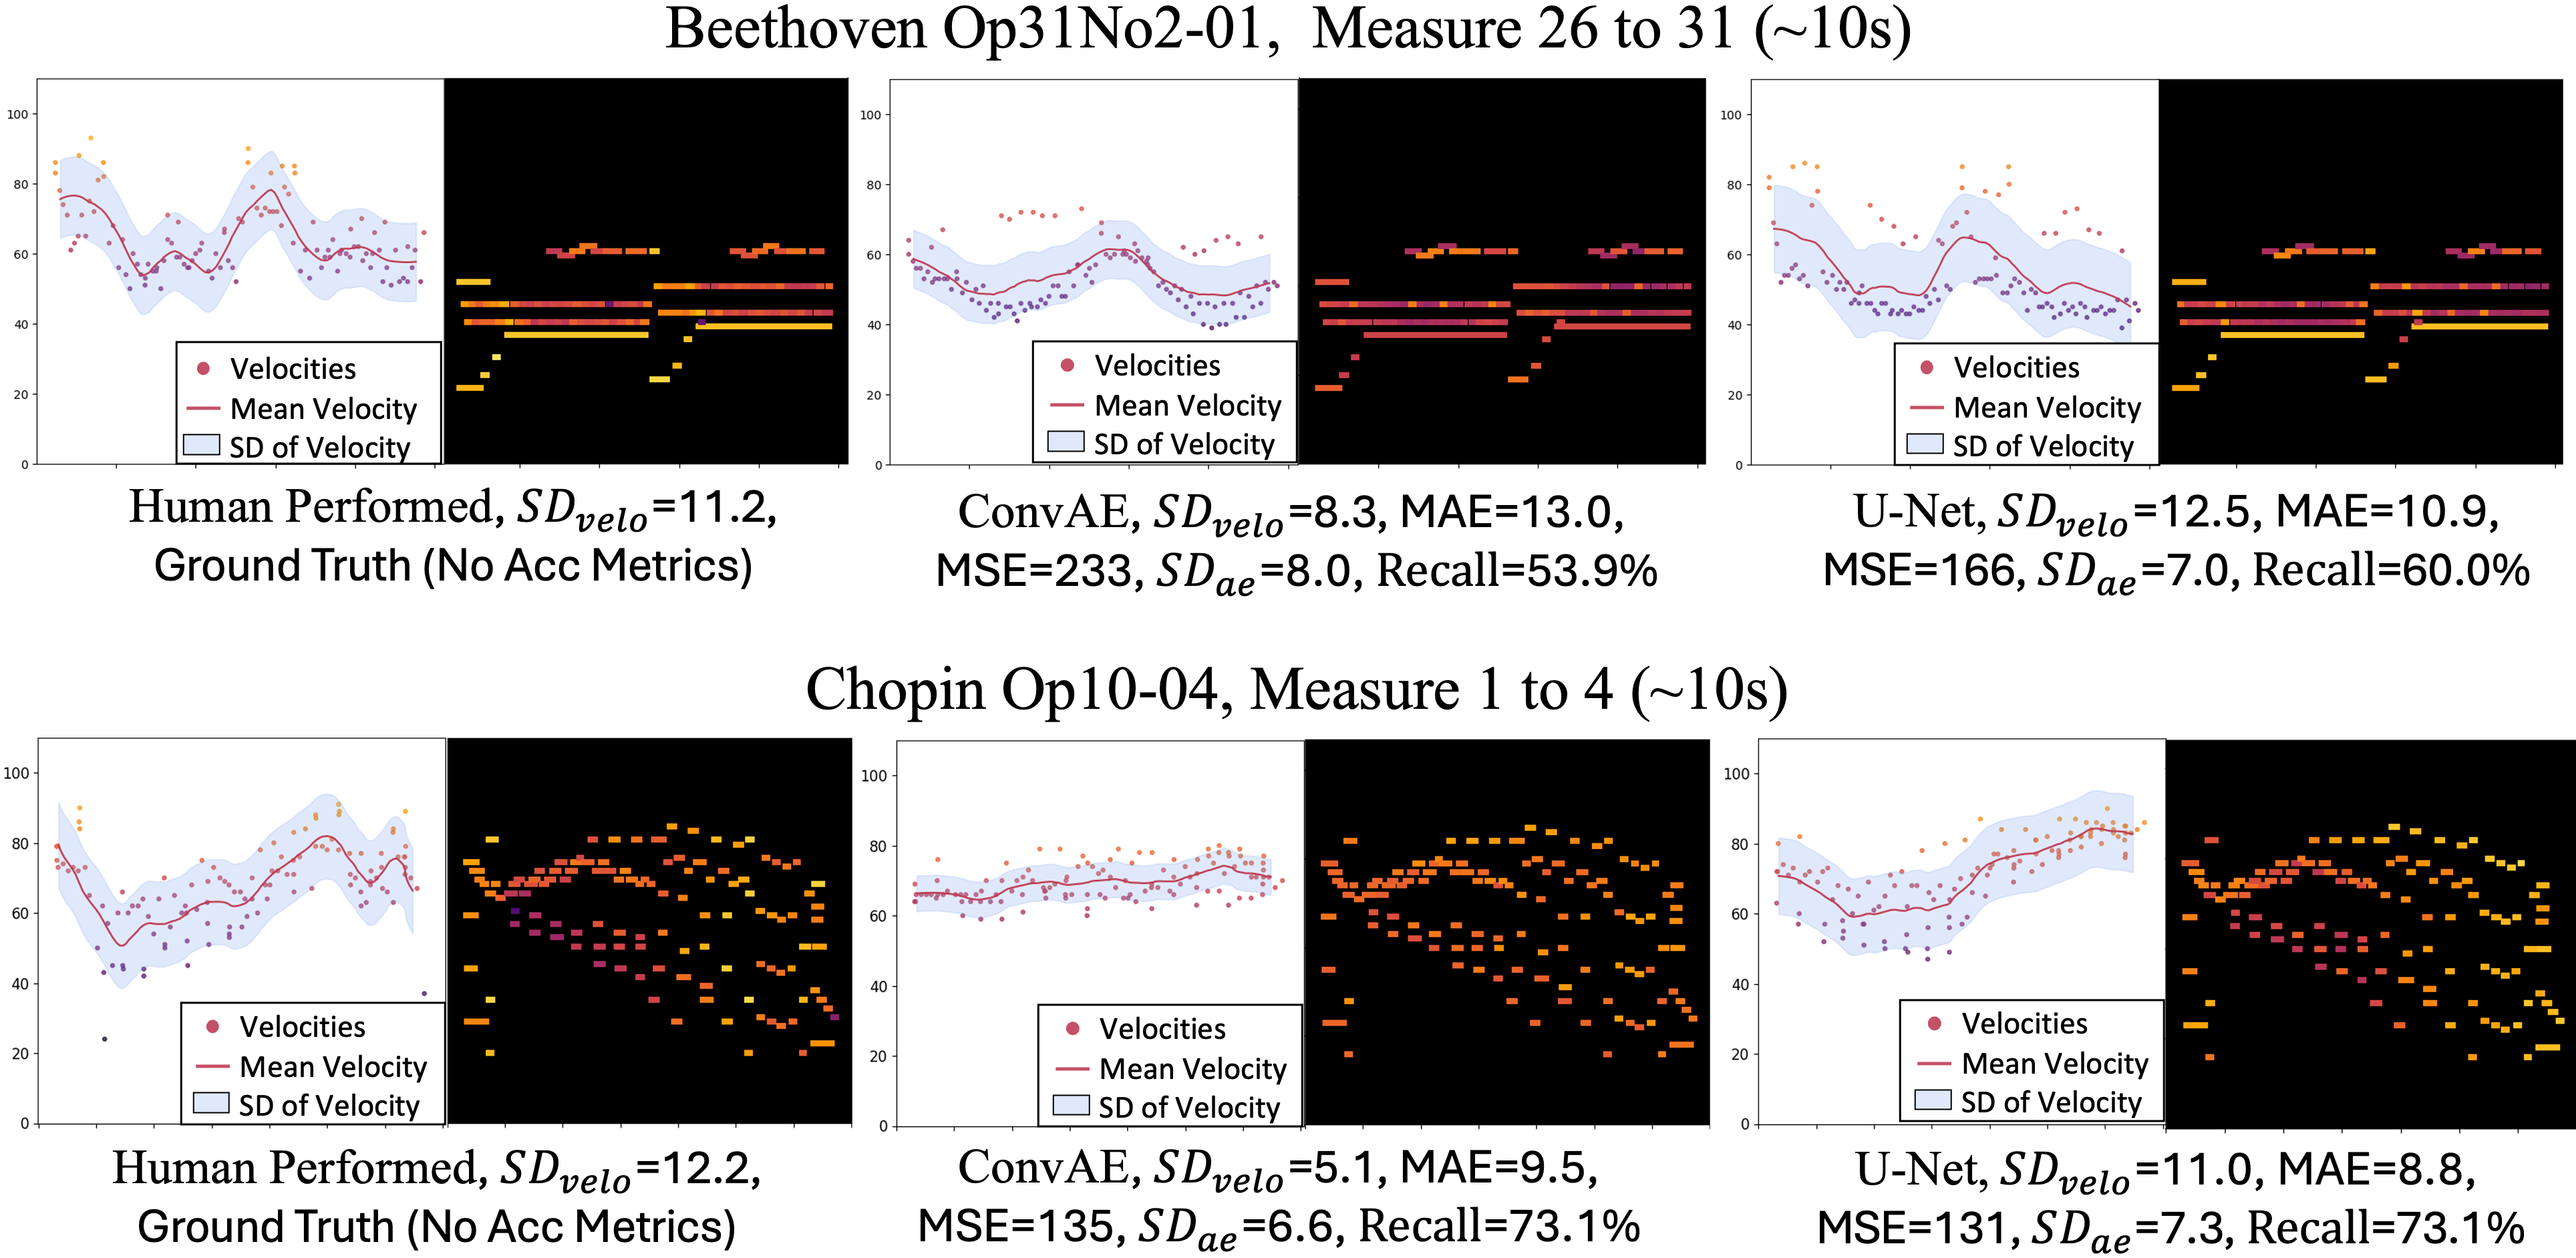
\includegraphics[width=\columnwidth]{Chapter_3/figures/p4v1.png}
\caption{Comparison of human-performed velocity with ConvAE and U-Net predictions. The U-Net result is more human-like than ConvAE, but for Chopin Op.~10 No.~4 the standard accuracy metrics do not fully reflect this difference.}
\label{fig:velcomp_visual}
\end{center}
\end{figure}

The metric behavior warrants some discussion. When the predictions are visualized, as in Figure~\ref{fig:velcomp_visual}, two patterns become clear. First, accuracy metrics such as MAE, MSE, \(SD_{\mathrm{ae}}\), and Recall\textsubscript{10\%} usually distinguish the models well, but there are cases in which they fail to reflect perceptual differences. The Chopin Op.~10 No.~4 excerpt is one such example, where a mid-range local optimum produces superficially acceptable error values. Second, \(SD_{\mathrm{velo}}\) is especially informative because it reflects the dispersion of predicted velocities around their mean. Higher values tend to reveal clearer differentiation between the hands and therefore a more human-like intensity profile.


\section{Ablation Summary}
Table \ref{tb:result_maestro} presents an ablation study evaluating key components of the proposed U-Net model.

\begin{table*}[h!]
\centering
% \scriptsize                        % 控制字体, 把字体切到 LaTeX 预定义的小字号
\setlength{\tabcolsep}{1.5pt}          % 控制表格列与列之间的左右留白
\fontsize{11pt}{12pt}\selectfont     % 直接设置字体大小和行高
\renewcommand{\arraystretch}{1.2}    % 控制表格行高倍率
% 调整结束
\begin{tabular}{llll|ccccc}
\toprule
\multirow{2}{*}{\textbf{Model}} &
\multirow{2}{*}{\textbf{Attn.}} &
\multirow{2}{*}{\textbf{Dur.}} &
\multirow{2}{*}{\textbf{Loss}} &
\multicolumn{5}{c}{\textbf{MAESTRO test set}} \\
\cmidrule(l){5-9}
& & & &
\textbf{MAE \(\downarrow\)} &
\textbf{MSE \(\downarrow\)} &
\textbf{SD\textsubscript{ae} \(\downarrow\)} &
\textbf{Recall\textsubscript{10\%} \(\uparrow\)} &
\textbf{SD\textsubscript{velo} \(\uparrow\)} \\
\midrule
U-Net & 1x1     & 10s & Comb $<m,w>$ & 11.7 & 237.7 & 9.7 & 62.3\% & 10.3\\
\textbf{U-Net*} & \textbf{2x2} & \textbf{10s} & \textbf{Comb $<m,w>$} & \textbf{11.5} & \textbf{226.2} & \textbf{9.4} & \textbf{63.8\%} & 10.7\\
U-Net & 4x4     & 10s & Comb $<m,w>$ & 11.6 & 230.5 & 9.5 & 63.3\% & 10.7\\
U-Net & 8x8     & 10s & Comb $<m,w>$ & 11.7 & 233.0 & 9.6 & 62.8\% & 10.6\\
U-Net & no attn & 10s & Comb $<m,w>$ & 12.3 & 252.5 & 10.0 & 61.3\% & 9.9\\
\midrule
U-Net & 2x2     & 5s  & Comb $<m,w>$ & 11.6 & 229.2 & 9.5 & 63.3\% & 11.0\\
U-Net & 2x2     & 15s & Comb $<m,w>$ & 11.6 & 231.9 & 9.5 & 63.1\% & 10.5\\
U-Net & 2x2     & 20s & Comb $<m,w>$ & 12.0 & 244.8 & 9.9 & 61.5\% & 10.6\\
\midrule
U-Net & 2x2     & 10s & BCE          & 13.6 & 304.5 & 10.7 & 55.0\% & \textbf{12.8} \\
U-Net & 2x2     & 10s & BCE $<m>$    & 11.6 & 228.2 & 9.4 & 63.4\% & 10.0 \\
U-Net & 2x2     & 10s & BCE $<m,w>$  & 11.5 & 227.6 & 9.4 & 63.6\% & 10.9 \\
\bottomrule
\end{tabular}
\caption{Ablation study on the MAESTRO test set. \(Attn.\) denotes component ablation by adjusting the attention window, or removing attention. \(Dur.\) represents the MIDI segment duration, $<m,w>$ indicates loss with masking and weighting. An asterisk * marks the best configuration used for quantitative evaluation.}
\label{tb:result_maestro}
\end{table*}


\textbf{Window attention mechanism.} We evaluated different attention configurations to assess their impact. Removing attention reduced performance, which highlighted the attention mechanism's role in focusing on salient features and improved U-Net's performance. The 1×1 window attention (i.e., global attention) was tested alongside \{2×2, 4×4, 8×8\} windows, with GPU memory requirements gradually reducing. Among these, 2×2 window attention performed best. The result shows that while window attention mitigates MIDI sparsity, large windows over-compress information, reducing effectiveness.

\textbf{MIDI segment duration.} The analysis shows that reducing it from 20 to 10 seconds improves performance, while further reduction to 5 seconds slightly worsens the accuracy metrics. This is likely because a 10-second segment roughly encompasses four measures at 120 beats per minute (BPM), forming a complete musical phrase that aids in semantic segmentation.

\textbf{Loss function.} Training with BCE loss alone produced a wide velocity dispersion (highest \(SD_{\text{velo}}\)), but this came with the lowest accuracy metrics. Applying the masking $<m>$ improved accuracy but reduced \(SD_{\text{velo}}\) as a trade-off. The weighting $<w>$ encouraged predictions to deviate from the mean, increasing both \(SD_{\text{velo}}\) and accuracy metrics. Finally, adding CosSim achieved the highest overall accuracy, with a negligible drop in \(SD_{\text{velo}}\). This combined loss function $\mathcal{L}_{\mathrm{Comb}}^{<m,w>}$ was recognized as the optimal configuration and applied in the training of both U-Net and ConvAE.

% The application of masking $<m>$ and CosSim improves model accuracy, leading to lower MAE, MSE, and \(SD_{\text{ae}}\), as well as better Recall. Meanwhile, the weighting $<w>$ introduces a more dispersed velocity distribution, reflected in a higher \(SD_{\text{velo}}\). The final combined loss achieves optimal overall performance across all metrics.



\section{Perceptual Evaluation}
\label{sec:velcomp:perceptual}

A MUSHRA-inspired reference-based listening test was conducted to evaluate the human-likeness of performances generated by U-Net, ConvAE \cite{kuo2021velocity}, and the Flat model.

\paragraph{Participants.}
We recruited 11 expert listeners aged 18 or above, selected for substantial musical background and experience with critical listening studies.
Participants completed the survey anonymously through the Qualtrics platform \cite{qualtrics}.

\paragraph{Stimuli.}
The test used eight 10-second MIDI segments, each selected from one of the SMD performances listed in Table~\ref{tab:velcomp_composers}.
For each segment, the original human-performed velocities were removed to create a common symbolic input.
The Flat, ConvAE, and U-Net outputs were then rendered as stimuli, while the original MIDI with human-performed velocity served as the reference.
All stimuli were rendered with the PianoTeq~8 plug-in using the Steinway Model D instrument.

\paragraph{Calibration.}
The dataset also provides corresponding recordings from the Yamaha Disklavier used in performance, which approximate what the pianist heard.
To render the MIDI as faithfully as possible, we calibrated the PianoTeq~8 dynamics control against those recordings.
Calibration compared momentary loudness correlation and loudness range, following BS.1770/EBU R128.
The results in Table~\ref{tab:velcomp_pianoteq} show that a dynamics setting of 60~dB best matched the original recordings, and this setting was used for all listening-test stimuli.

\begin{table}[t]
\centering
% \scriptsize                        % 控制字体, 把字体切到 LaTeX 预定义的小字号
\setlength{\tabcolsep}{7pt}          % 控制表格列与列之间的左右留白
\fontsize{11pt}{14pt}\selectfont     % 直接设置字体大小和行高
\renewcommand{\arraystretch}{1.2}    % 控制表格行高倍率
\caption{Metrics for comparing different PianoTeq configurations against the reference recordings.}
\label{tab:velcomp_pianoteq}
\begin{tabular}{|l|c|c|}
\hline
\textbf{Dynamics (dB)} & \textbf{Loudness $\Delta$ \(\downarrow\)} & \textbf{Correlation Coefficient \(\uparrow\)} \\
\hline
50 & 1.8 & 0.9583 \\
\hline
\textbf{60} & \textbf{0.3} & \textbf{0.9591} \\
\hline
70 & 0.9 & 0.9561 \\
\hline
80 & 1.9 & 0.9535 \\
\hline
90 & 3.1 & 0.9479 \\
\hline
\end{tabular}
\end{table}

\paragraph{Procedure.}
Participants were instructed to use headphones because the relevant velocity differences are subtle and are easier to judge at adequate playback quality and level.
In each trial, the audio rendered from the human-performed MIDI served as the fixed reference, and the rendered system outputs were judged relative to that reference.
Following a MUSHRA-inspired reference-based procedure \cite{series2014mursha}, participants rated each processed stimulus independently on a continuous 0--5 scale, where the labeled intervals corresponded to ``bad'', ``poor'', ``fair'', ``good'', and ``excellent'' similarity.
The final scores were averaged across listeners to obtain MOS, and 95\% confidence intervals were computed for reporting.

\begin{table}[t]
\centering
\caption{Listening-test results. MOS values with 95\% confidence intervals are reported. ``Most seen'' composers include \{Chopin, Bach, Beethoven\}; ``less seen'' composers include \{Rachmaninoff, Haydn, Mozart\}; and ``unseen'' composers include \{Bart\'ok, Ravel\}.}
\label{tab:velcomp_mos}
% \scriptsize                        % 控制字体, 把字体切到 LaTeX 预定义的小字号
\setlength{\tabcolsep}{7pt}          % 控制表格列与列之间的左右留白
\fontsize{11pt}{13pt}\selectfont     % 直接设置字体大小和行高
\renewcommand{\arraystretch}{1.2}    % 控制表格行高倍率
% 调整结束
\begin{tabular}{l|cccc}
\toprule
\multicolumn{1}{c|}{\multirow{2}{*}{\textbf{Model}}}
& \multicolumn{4}{c}{\textbf{SMD dataset (selected corpus)}} \\
\cmidrule(l){2-5}
& \makecell{\textbf{Most Seen}\\\textbf{Compo. MOS} \(\uparrow\)}
& \makecell{\textbf{Less Seen}\\\textbf{Compo. MOS} \(\uparrow\)}
& \makecell{\textbf{Unseen}\\\textbf{Compo. MOS} \(\uparrow\)}
& \makecell{\textbf{Overall}\\\textbf{MOS} \(\uparrow\)} \\
\midrule
Flat & $1.58 \pm 0.36$ & $1.64 \pm 0.44$ & $1.18 \pm 0.42$ & $1.50 \pm 0.37$ \\
ConvAE & $1.93 \pm 0.34$ & $2.40 \pm 0.39$ & $1.80 \pm 0.44$ & $2.08 \pm 0.33$ \\
\textbf{U-Net} & $\mathbf{3.10 \pm 0.38}$ & $\mathbf{3.16 \pm 0.29}$ & $\mathbf{2.67 \pm 0.46}$ & $\mathbf{3.01 \pm 0.34}$ \\
\bottomrule
\end{tabular}
\end{table}

\paragraph{Results.}
Although a substantial gap to human performance remains, the proposed U-Net clearly outperforms the other systems.
The Flat model performs worst, consistent with earlier findings that default velocity is musically inadequate \cite{kuo2021velocity}.
One limitation of the listening test is that differences between seen and unseen repertoire cannot be cleanly separated from differences in musical complexity.
Even so, the relatively narrow 95\% confidence intervals across groups suggest that participants rated the stimuli with reasonable consistency.

\section{Discussion}
\label{sec:velcomp:discussion}

This chapter makes a focused thesis-level point: note-level dynamics can be recovered usefully even when the symbolic notes and timing are held fixed.
That narrow formulation matters.
It turns expressive enhancement into a controllable post-processing stage rather than a full performance-rendering problem, which is exactly the setting encountered in many MIDI-production and corpus-curation workflows.

The image-colorization view is effective because it matches the structure of the data.
Polyphonic note patterns create meaningful vertical and local spatial regularities that are awkward to express in purely sequential terms.
The U-Net captures this local structure well, and the sparsity-aware loss prevents the model from spending most of its capacity on silent regions.
The results suggest that this representation choice is a major reason the method surpasses the sequence-based baselines considered here.

At the same time, the chapter also exposes clear limits.
Objective error metrics alone do not fully capture musical plausibility, which is why the listening test and the dispersion-sensitive statistic \(SD_{\mathrm{velo}}\) are important.
Qualitative inspection further suggests that the remaining errors are most noticeable in dense chordal textures, fast ornaments, and passages that require stronger excursions toward the extremes of the velocity range.
The boundary-weighted loss helps with these cases, but it does not eliminate them.

The most important external limitation is scope.
All experiments are performed on piano datasets recorded with Yamaha Disklavier instruments.
The cross-dataset MAESTRO-to-SMD results are encouraging, but they do not yet establish robustness across instruments or across substantially different capture conditions.
This limitation motivates the later thesis chapters on score-informed correction and extension beyond piano.
In other words, the present chapter is intentionally narrow: it solves the symbolic-only velocity-completion problem as a clean and practical building block for the broader expressive-data curation pipeline.


In the language of Chapter~\ref{ch:background}, this chapter primarily addresses Requirement~R1 by preserving note content and timing, and Requirement~R2 under the symbolic-only regime. It also contributes to Requirement~R5 by combining objective metrics with perceptual evaluation. The chapter does not solve cross-instrument transfer or score-level interpretation, but it establishes a clean and practical baseline: note-level dynamics recovery is already useful before audio or score information is introduced.

% ===== THESIS TODO (recommended final addition) =====
% Add one short qualitative failure case from a dense passage or fast ornamented excerpt.
% Suggested thesis-facing conclusion: the current model is strongest when local polyphonic texture is stable,
% and it remains weaker when expressive intent requires broader phrase planning or more extreme velocity excursions.
